% Options for packages loaded elsewhere
% Options for packages loaded elsewhere
\PassOptionsToPackage{unicode,hidelinks}{hyperref}
\PassOptionsToPackage{hyphens}{url}
\PassOptionsToPackage{dvipsnames,svgnames,x11names}{xcolor}
%
\documentclass[
  american,
  12pt,
  letterpaper,
]{article}
\usepackage{xcolor}
\usepackage[margin=1in]{geometry}
\usepackage{amsmath,amssymb}
\setcounter{secnumdepth}{-\maxdimen} % remove section numbering
\usepackage{iftex}
\ifPDFTeX
  \usepackage[T1]{fontenc}
  \usepackage[utf8]{inputenc}
  \usepackage{textcomp} % provide euro and other symbols
\else % if luatex or xetex
  \usepackage{unicode-math} % this also loads fontspec
  \defaultfontfeatures{Scale=MatchLowercase}
  \defaultfontfeatures[\rmfamily]{Ligatures=TeX,Scale=1}
\fi
\usepackage{lmodern}
\ifPDFTeX\else
  % xetex/luatex font selection
  \setmainfont[]{Times New Roman}
\fi
% Use upquote if available, for straight quotes in verbatim environments
\IfFileExists{upquote.sty}{\usepackage{upquote}}{}
\IfFileExists{microtype.sty}{% use microtype if available
  \usepackage[]{microtype}
  \UseMicrotypeSet[protrusion]{basicmath} % disable protrusion for tt fonts
}{}

\usepackage{color}
\usepackage{fancyvrb}
\newcommand{\VerbBar}{|}
\newcommand{\VERB}{\Verb[commandchars=\\\{\}]}
\DefineVerbatimEnvironment{Highlighting}{Verbatim}{commandchars=\\\{\}}
% Add ',fontsize=\small' for more characters per line
\usepackage{framed}
\definecolor{shadecolor}{RGB}{241,243,245}
\newenvironment{Shaded}{\begin{snugshade}}{\end{snugshade}}
\newcommand{\AlertTok}[1]{\textcolor[rgb]{0.68,0.00,0.00}{#1}}
\newcommand{\AnnotationTok}[1]{\textcolor[rgb]{0.37,0.37,0.37}{#1}}
\newcommand{\AttributeTok}[1]{\textcolor[rgb]{0.40,0.45,0.13}{#1}}
\newcommand{\BaseNTok}[1]{\textcolor[rgb]{0.68,0.00,0.00}{#1}}
\newcommand{\BuiltInTok}[1]{\textcolor[rgb]{0.00,0.23,0.31}{#1}}
\newcommand{\CharTok}[1]{\textcolor[rgb]{0.13,0.47,0.30}{#1}}
\newcommand{\CommentTok}[1]{\textcolor[rgb]{0.37,0.37,0.37}{#1}}
\newcommand{\CommentVarTok}[1]{\textcolor[rgb]{0.37,0.37,0.37}{\textit{#1}}}
\newcommand{\ConstantTok}[1]{\textcolor[rgb]{0.56,0.35,0.01}{#1}}
\newcommand{\ControlFlowTok}[1]{\textcolor[rgb]{0.00,0.23,0.31}{\textbf{#1}}}
\newcommand{\DataTypeTok}[1]{\textcolor[rgb]{0.68,0.00,0.00}{#1}}
\newcommand{\DecValTok}[1]{\textcolor[rgb]{0.68,0.00,0.00}{#1}}
\newcommand{\DocumentationTok}[1]{\textcolor[rgb]{0.37,0.37,0.37}{\textit{#1}}}
\newcommand{\ErrorTok}[1]{\textcolor[rgb]{0.68,0.00,0.00}{#1}}
\newcommand{\ExtensionTok}[1]{\textcolor[rgb]{0.00,0.23,0.31}{#1}}
\newcommand{\FloatTok}[1]{\textcolor[rgb]{0.68,0.00,0.00}{#1}}
\newcommand{\FunctionTok}[1]{\textcolor[rgb]{0.28,0.35,0.67}{#1}}
\newcommand{\ImportTok}[1]{\textcolor[rgb]{0.00,0.46,0.62}{#1}}
\newcommand{\InformationTok}[1]{\textcolor[rgb]{0.37,0.37,0.37}{#1}}
\newcommand{\KeywordTok}[1]{\textcolor[rgb]{0.00,0.23,0.31}{\textbf{#1}}}
\newcommand{\NormalTok}[1]{\textcolor[rgb]{0.00,0.23,0.31}{#1}}
\newcommand{\OperatorTok}[1]{\textcolor[rgb]{0.37,0.37,0.37}{#1}}
\newcommand{\OtherTok}[1]{\textcolor[rgb]{0.00,0.23,0.31}{#1}}
\newcommand{\PreprocessorTok}[1]{\textcolor[rgb]{0.68,0.00,0.00}{#1}}
\newcommand{\RegionMarkerTok}[1]{\textcolor[rgb]{0.00,0.23,0.31}{#1}}
\newcommand{\SpecialCharTok}[1]{\textcolor[rgb]{0.37,0.37,0.37}{#1}}
\newcommand{\SpecialStringTok}[1]{\textcolor[rgb]{0.13,0.47,0.30}{#1}}
\newcommand{\StringTok}[1]{\textcolor[rgb]{0.13,0.47,0.30}{#1}}
\newcommand{\VariableTok}[1]{\textcolor[rgb]{0.07,0.07,0.07}{#1}}
\newcommand{\VerbatimStringTok}[1]{\textcolor[rgb]{0.13,0.47,0.30}{#1}}
\newcommand{\WarningTok}[1]{\textcolor[rgb]{0.37,0.37,0.37}{\textit{#1}}}

\usepackage{longtable,booktabs,array}
\newcounter{none} % for unnumbered tables
\usepackage{calc} % for calculating minipage widths
% Correct order of tables after \paragraph or \subparagraph
\usepackage{etoolbox}
\makeatletter
\patchcmd\longtable{\par}{\if@noskipsec\mbox{}\fi\par}{}{}
\makeatother
% Allow footnotes in longtable head/foot
\IfFileExists{footnotehyper.sty}{\usepackage{footnotehyper}}{\usepackage{footnote}}
\makesavenoteenv{longtable}
\usepackage{graphicx}
\makeatletter
\newsavebox\pandoc@box
\newcommand*\pandocbounded[1]{% scales image to fit in text height/width
  \sbox\pandoc@box{#1}%
  \Gscale@div\@tempa{\textheight}{\dimexpr\ht\pandoc@box+\dp\pandoc@box\relax}%
  \Gscale@div\@tempb{\linewidth}{\wd\pandoc@box}%
  \ifdim\@tempb\p@<\@tempa\p@\let\@tempa\@tempb\fi% select the smaller of both
  \ifdim\@tempa\p@<\p@\scalebox{\@tempa}{\usebox\pandoc@box}%
  \else\usebox{\pandoc@box}%
  \fi%
}
% Set default figure placement to htbp
\def\fps@figure{htbp}
\makeatother


% definitions for citeproc citations
\NewDocumentCommand\citeproctext{}{}
\NewDocumentCommand\citeproc{mm}{%
  \begingroup\def\citeproctext{#2}\cite{#1}\endgroup}
\makeatletter
 % allow citations to break across lines
 \let\@cite@ofmt\@firstofone
 % avoid brackets around text for \cite:
 \def\@biblabel#1{}
 \def\@cite#1#2{{#1\if@tempswa , #2\fi}}
\makeatother
\newlength{\cslhangindent}
\setlength{\cslhangindent}{1.5em}
\newlength{\csllabelwidth}
\setlength{\csllabelwidth}{3em}
\newenvironment{CSLReferences}[2] % #1 hanging-indent, #2 entry-spacing
 {\begin{list}{}{%
  \setlength{\itemindent}{0pt}
  \setlength{\leftmargin}{0pt}
  \setlength{\parsep}{0pt}
  % turn on hanging indent if param 1 is 1
  \ifodd #1
   \setlength{\leftmargin}{\cslhangindent}
   \setlength{\itemindent}{-1\cslhangindent}
  \fi
  % set entry spacing
  \setlength{\itemsep}{#2\baselineskip}}}
 {\end{list}}
\usepackage{calc}
\newcommand{\CSLBlock}[1]{\hfill\break\parbox[t]{\linewidth}{\strut\ignorespaces#1\strut}}
\newcommand{\CSLLeftMargin}[1]{\parbox[t]{\csllabelwidth}{\strut#1\strut}}
\newcommand{\CSLRightInline}[1]{\parbox[t]{\linewidth - \csllabelwidth}{\strut#1\strut}}
\newcommand{\CSLIndent}[1]{\hspace{\cslhangindent}#1}

\ifLuaTeX
\usepackage[bidi=basic,shorthands=off]{babel}
\else
\usepackage[bidi=default,shorthands=off]{babel}
\fi
\ifPDFTeX
\else
\babelfont{rm}[]{Times New Roman}
\fi
\ifLuaTeX
  \usepackage{selnolig} % disable illegal ligatures
\fi


\setlength{\emergencystretch}{3em} % prevent overfull lines

\providecommand{\tightlist}{%
  \setlength{\itemsep}{0pt}\setlength{\parskip}{0pt}}



 


\usepackage{setspace}
\usepackage{fancyhdr}
\usepackage{titlesec}
\usepackage{indentfirst}

% ========================================================
% BODY
% ========================================================

\doublespacing

\setlength{\parindent}{0.5in}
\setlength{\parskip}{0pt}

% ========================================================
% PAGE NUMBERS
%
% Title page:
%   no visible number
%
% First actual text page:
%   Arabic page 1, upper right
% ========================================================

\setlength{\headheight}{15pt}

\pagestyle{fancy}
\fancyhf{}
\fancyhead[R]{\thepage}

\renewcommand{\headrulewidth}{0pt}
\renewcommand{\footrulewidth}{0pt}

\fancypagestyle{plain}{
  \fancyhf{}
  \fancyhead[R]{\thepage}
  \renewcommand{\headrulewidth}{0pt}
  \renewcommand{\footrulewidth}{0pt}
}

% ========================================================
% FIVE-LEVEL HEADING SYSTEM
%
% Level 1 = centered, bold
% Level 2 = centered, regular
% Level 3 = flush left, italic
% Level 4 = flush left, regular
% Level 5 = run-in, italic, terminal period
% ========================================================

\titleformat{\section}[block]
  {\normalfont\normalsize\bfseries\centering}
  {}
  {0pt}
  {}

\titleformat{\subsection}[block]
  {\normalfont\normalsize\centering}
  {}
  {0pt}
  {}

\titleformat{\subsubsection}[block]
  {\normalfont\normalsize\itshape}
  {}
  {0pt}
  {}

\titleformat{\paragraph}[block]
  {\normalfont\normalsize}
  {}
  {0pt}
  {}

\titleformat{\subparagraph}[runin]
  {\normalfont\normalsize\itshape}
  {}
  {0pt}
  {}
  [.]

% ========================================================
% HEADING SPACING
% ========================================================

\titlespacing{\section}
  {0pt}
  {\baselineskip}
  {\baselineskip}

\titlespacing{\subsection}
  {0pt}
  {\baselineskip}
  {\baselineskip}

\titlespacing{\subsubsection}
  {0pt}
  {\baselineskip}
  {\baselineskip}

\titlespacing{\paragraph}
  {0pt}
  {\baselineskip}
  {\baselineskip}

\titlespacing{\subparagraph}
  {0pt}
  {\baselineskip}
  {0.5em}

% ========================================================
% BLOCK QUOTATIONS
%
% Single spaced internally.
% 0.5-inch left indent.
% Same 12-point type.
% ========================================================

\renewenvironment{quote}
  {
    \par
    \addvspace{\baselineskip}
    \begin{singlespace}
    \begin{list}{}{%
      \setlength{\leftmargin}{0.5in}%
      \setlength{\rightmargin}{0in}%
      \setlength{\topsep}{0pt}%
      \setlength{\partopsep}{0pt}%
      \setlength{\parsep}{0pt}%
      \setlength{\itemsep}{0pt}%
    }
    \item\relax
  }
  {
    \end{list}
    \end{singlespace}
    \par
    \addvspace{\baselineskip}
  }

% ========================================================
% REFERENCES
%
% 0.5-inch hanging indent.
% CSL controls spacing between entries.
% ========================================================

\setlength{\cslhangindent}{0.5in}

\renewenvironment{CSLReferences}[2]
  {\begin{list}{}{%
    \setlength{\itemindent}{0pt}%
    \setlength{\leftmargin}{0pt}%
    \setlength{\rightmargin}{0pt}%
    \setlength{\parsep}{0pt}%
    \setlength{\topsep}{0pt}%
    \setlength{\partopsep}{0pt}%
    \ifodd #1%
      \setlength{\leftmargin}{\cslhangindent}%
      \setlength{\itemindent}{-1\cslhangindent}%
    \fi%
    \setlength{\itemsep}{#2\baselineskip}%
  }}
  {\end{list}}
\makeatletter
\@ifpackageloaded{caption}{}{\usepackage{caption}}
\AtBeginDocument{%
\ifdefined\contentsname
  \renewcommand*\contentsname{Table of contents}
\else
  \newcommand\contentsname{Table of contents}
\fi
\ifdefined\listfigurename
  \renewcommand*\listfigurename{List of Figures}
\else
  \newcommand\listfigurename{List of Figures}
\fi
\ifdefined\listtablename
  \renewcommand*\listtablename{List of Tables}
\else
  \newcommand\listtablename{List of Tables}
\fi
\ifdefined\figurename
  \renewcommand*\figurename{Figure}
\else
  \newcommand\figurename{Figure}
\fi
\ifdefined\tablename
  \renewcommand*\tablename{Table}
\else
  \newcommand\tablename{Table}
\fi
}
\@ifpackageloaded{float}{}{\usepackage{float}}
\floatstyle{ruled}
\@ifundefined{c@chapter}{\newfloat{codelisting}{h}{lop}}{\newfloat{codelisting}{h}{lop}[chapter]}
\floatname{codelisting}{Listing}
\newcommand*\listoflistings{\listof{codelisting}{List of Listings}}
\makeatother
\makeatletter
\makeatother
\makeatletter
\@ifpackageloaded{caption}{}{\usepackage{caption}}
\@ifpackageloaded{subcaption}{}{\usepackage{subcaption}}
\makeatother
\usepackage{bookmark}
\IfFileExists{xurl.sty}{\usepackage{xurl}}{} % add URL line breaks if available
\urlstyle{same}
% fallback for those not using the hyperref driver hyperxmp:
\makeatletter
\@ifundefined{xmpquote}{\newcommand{\xmpquote}[1]{#1}}{}
\makeatother
\hypersetup{
  pdflang={en-US},
  colorlinks=true,
  linkcolor={blue},
  filecolor={Maroon},
  citecolor={Blue},
  urlcolor={Blue},
  pdfcreator={LaTeX via pandoc}}


\author{}
\date{}
\begin{document}


\begin{titlepage}

\thispagestyle{empty}

% Title approximately one-third down the physical page.

\vspace*{0.30\textheight}

{\centering

Your Paper Title\par

% Purdue says the identifying information should appear
% "several lines later."
%
% Eight double-spaced baselines is being used as a visual
% implementation of the sample, not as an independent
% Chicago rule.

\vspace{8\baselineskip}

Your Name\par
Course Number: Course Name\par
Month Day, Year\par

}

\end{titlepage}

% First page of actual text = page 1.

\setcounter{page}{1}

Start writing your paper here. Normal body text is 12-point Times New
Roman, double-spaced, with one-inch margins in paged document formats
and a half-inch first-line paragraph indent.

A standard Chicago 18 author-date citation looks like this (Smith 2024,
42).

Another source can be cited like this (Jones 2022, 220).

For a narrative citation, Smith (2024, 42) argues that the evidence
supports this interpretation.

This is another paragraph so you can verify ordinary paragraph
indentation and line spacing.

\begin{Shaded}
\begin{Highlighting}[]
\ControlFlowTok{if}\NormalTok{ (}\SpecialCharTok{!}\FunctionTok{require}\NormalTok{(}\StringTok{"pacman"}\NormalTok{)) }
  \FunctionTok{install.packages}\NormalTok{(}\StringTok{"pacman"}\NormalTok{)}
\end{Highlighting}
\end{Shaded}

\begin{verbatim}
Loading required package: pacman
\end{verbatim}

\begin{Shaded}
\begin{Highlighting}[]
\FunctionTok{library}\NormalTok{(pacman)}

\NormalTok{pacman}\SpecialCharTok{::}\FunctionTok{p\_load}\NormalTok{(}
\NormalTok{  ggplot2,}
\NormalTok{  ggtext}
\NormalTok{)}

\NormalTok{knitr}\SpecialCharTok{::}\NormalTok{opts\_chunk}\SpecialCharTok{$}\FunctionTok{set}\NormalTok{(}\AttributeTok{dev =} \StringTok{"ragg\_png"}\NormalTok{)}
\end{Highlighting}
\end{Shaded}

\begin{Shaded}
\begin{Highlighting}[]
\CommentTok{\# https://advance.lexis.com/api/permalink/5bbd017c{-}bb50{-}4cb5{-}a4fa{-}0d2066a1d2de/?context=1519360\&identityprofileid=BQ226N51782}

\NormalTok{DATA\_FILE }\OtherTok{\textless{}{-}} \StringTok{"CoverageoverTime\_FlockcameraORFlockcamerasORFlockSafety.csv"}

\NormalTok{lexis\_coverage\_raw }\OtherTok{\textless{}{-}} \FunctionTok{read.csv2}\NormalTok{(}
\NormalTok{  DATA\_FILE,}
  \AttributeTok{check.names =} \ConstantTok{FALSE}\NormalTok{,}
  \AttributeTok{fileEncoding =} \StringTok{"UTF{-}8{-}BOM"}
\NormalTok{)}

\NormalTok{lexis\_coverage\_monthly }\OtherTok{\textless{}{-}} \FunctionTok{data.frame}\NormalTok{(}
  \AttributeTok{month =} \FunctionTok{as.Date}\NormalTok{(}\FunctionTok{substr}\NormalTok{(}
\NormalTok{    lexis\_coverage\_raw[[}\StringTok{"Coverage over Time"}\NormalTok{]], }\DecValTok{1}\NormalTok{, }\DecValTok{10}
\NormalTok{  )),}
  \AttributeTok{articles =} \FunctionTok{as.integer}\NormalTok{(lexis\_coverage\_raw[[}\StringTok{"Coverage"}\NormalTok{]])}
\NormalTok{)}

\NormalTok{lexis\_coverage\_complete }\OtherTok{\textless{}{-}} \FunctionTok{subset}\NormalTok{(}
\NormalTok{  lexis\_coverage\_monthly,}
\NormalTok{  month }\SpecialCharTok{\textless{}=} \FunctionTok{as.Date}\NormalTok{(}\StringTok{"2026{-}08{-}01"}\NormalTok{)}
\NormalTok{)}

\NormalTok{lexis\_coverage\_september\_segment }\OtherTok{\textless{}{-}} \FunctionTok{subset}\NormalTok{(}
\NormalTok{  lexis\_coverage\_monthly,}
\NormalTok{  month }\SpecialCharTok{\textgreater{}=} \FunctionTok{as.Date}\NormalTok{(}\StringTok{"2026{-}08{-}01"}\NormalTok{)}
\NormalTok{)}

\NormalTok{lexis\_coverage\_september }\OtherTok{\textless{}{-}} \FunctionTok{subset}\NormalTok{(}
\NormalTok{  lexis\_coverage\_monthly,}
\NormalTok{  month }\SpecialCharTok{==} \FunctionTok{as.Date}\NormalTok{(}\StringTok{"2026{-}09{-}01"}\NormalTok{)}
\NormalTok{)}

\NormalTok{plot\_lexis\_coverage\_monthly }\OtherTok{\textless{}{-}} \FunctionTok{ggplot}\NormalTok{(}
\NormalTok{  lexis\_coverage\_monthly,}
  \FunctionTok{aes}\NormalTok{(}\AttributeTok{x =}\NormalTok{ month, }\AttributeTok{y =}\NormalTok{ articles)}
\NormalTok{) }\SpecialCharTok{+}
  \FunctionTok{geom\_line}\NormalTok{(}
    \AttributeTok{data =}\NormalTok{ lexis\_coverage\_complete,}
    \AttributeTok{color =} \StringTok{"\#00A693"}\NormalTok{,}
    \AttributeTok{linewidth =} \DecValTok{1}
\NormalTok{  ) }\SpecialCharTok{+}
  \FunctionTok{geom\_line}\NormalTok{(}
    \AttributeTok{data =}\NormalTok{ lexis\_coverage\_september\_segment,}
    \AttributeTok{color =} \StringTok{"\#00A693"}\NormalTok{,}
    \AttributeTok{linewidth =} \DecValTok{1}\NormalTok{,}
    \AttributeTok{linetype =} \StringTok{"dashed"}
\NormalTok{  ) }\SpecialCharTok{+}
  \FunctionTok{geom\_point}\NormalTok{(}
    \AttributeTok{data =}\NormalTok{ lexis\_coverage\_complete,}
    \AttributeTok{color =} \StringTok{"\#00A693"}\NormalTok{,}
    \AttributeTok{size =} \FloatTok{2.3}
\NormalTok{  ) }\SpecialCharTok{+}
  \FunctionTok{geom\_point}\NormalTok{(}
    \AttributeTok{data =}\NormalTok{ lexis\_coverage\_september,}
    \AttributeTok{color =} \StringTok{"\#00A693"}\NormalTok{,}
    \AttributeTok{fill =} \StringTok{"white"}\NormalTok{,}
    \AttributeTok{shape =} \DecValTok{21}\NormalTok{,}
    \AttributeTok{size =} \FloatTok{2.8}\NormalTok{,}
    \AttributeTok{stroke =} \DecValTok{1}
\NormalTok{  ) }\SpecialCharTok{+}
  \FunctionTok{scale\_x\_date}\NormalTok{(}
    \AttributeTok{date\_breaks =} \StringTok{"1 month"}\NormalTok{,}
    \AttributeTok{date\_labels =} \StringTok{"\%b \%Y"}
\NormalTok{  ) }\SpecialCharTok{+}
  \FunctionTok{scale\_y\_continuous}\NormalTok{(}
    \AttributeTok{breaks =} \FunctionTok{c}\NormalTok{(}
      \FunctionTok{min}\NormalTok{(lexis\_coverage\_monthly}\SpecialCharTok{$}\NormalTok{articles),}
      \DecValTok{1000}\NormalTok{, }\DecValTok{2000}\NormalTok{, }\DecValTok{3000}\NormalTok{, }\DecValTok{4000}
\NormalTok{    ),}
    \AttributeTok{labels =}\NormalTok{ scales}\SpecialCharTok{::}\FunctionTok{label\_comma}\NormalTok{(),}
    \AttributeTok{limits =} \FunctionTok{c}\NormalTok{(}\FunctionTok{min}\NormalTok{(lexis\_coverage\_monthly}\SpecialCharTok{$}\NormalTok{articles), }\DecValTok{4500}\NormalTok{),}
    \AttributeTok{expand =} \FunctionTok{expansion}\NormalTok{(}\AttributeTok{mult =} \FunctionTok{c}\NormalTok{(}\DecValTok{0}\NormalTok{, }\DecValTok{0}\NormalTok{))}
\NormalTok{  ) }\SpecialCharTok{+}
  \FunctionTok{coord\_cartesian}\NormalTok{(}\AttributeTok{clip =} \StringTok{"off"}\NormalTok{) }\SpecialCharTok{+}
  \FunctionTok{labs}\NormalTok{(}
    \AttributeTok{title =} \FunctionTok{paste}\NormalTok{(}
      \StringTok{"News Articles Mentioning Flock"}\NormalTok{,}
      \AttributeTok{sep =} \StringTok{"}\SpecialCharTok{\textbackslash{}n}\StringTok{"}
\NormalTok{    ),}
    \AttributeTok{subtitle =} \StringTok{"Monthly Counts From a Nexis Uni News Search"}\NormalTok{,}
    \AttributeTok{x =} \ConstantTok{NULL}\NormalTok{,}
    \AttributeTok{y =} \StringTok{"Number of Articles"}\NormalTok{,}
    \AttributeTok{caption =} \FunctionTok{paste}\NormalTok{(}
      \StringTok{"\textless{}b\textgreater{}Source:\textless{}/b\textgreater{} Nexis Uni Analytics Export"}\NormalTok{,}
      \StringTok{"\textless{}b\textgreater{}Search Terms:\textless{}/b\textgreater{} Flock camera or Flock cameras or Flock Safety"}\NormalTok{,}
      \StringTok{"\textless{}b\textgreater{}Note:\textless{}/b\textgreater{} The dashed segment and open circle mark incomplete September results through September 27, 2026."}\NormalTok{,}
      \AttributeTok{sep =} \StringTok{"\textless{}br\textgreater{}"}
\NormalTok{    )}
\NormalTok{  ) }\SpecialCharTok{+}
  \FunctionTok{theme\_minimal}\NormalTok{(}
    \AttributeTok{base\_family =} \StringTok{"Georgia"}\NormalTok{,}
    \AttributeTok{base\_size =} \DecValTok{11}
\NormalTok{  ) }\SpecialCharTok{+}
  \FunctionTok{theme}\NormalTok{(}
    \AttributeTok{plot.title =} \FunctionTok{element\_text}\NormalTok{(}\AttributeTok{face =} \StringTok{"bold"}\NormalTok{, }\AttributeTok{size =} \DecValTok{14}\NormalTok{),}
    \AttributeTok{axis.text.x =} \FunctionTok{element\_text}\NormalTok{(}\AttributeTok{angle =} \DecValTok{45}\NormalTok{, }\AttributeTok{hjust =} \DecValTok{1}\NormalTok{),}
    \AttributeTok{panel.grid.minor =} \FunctionTok{element\_blank}\NormalTok{(),}
    \AttributeTok{panel.grid.major.x =} \FunctionTok{element\_blank}\NormalTok{(),}
    \AttributeTok{plot.caption =}\NormalTok{ ggtext}\SpecialCharTok{::}\FunctionTok{element\_markdown}\NormalTok{(}\AttributeTok{hjust =} \DecValTok{0}\NormalTok{, }\AttributeTok{size =} \DecValTok{9}\NormalTok{),}
    \AttributeTok{plot.caption.position =} \StringTok{"plot"}
\NormalTok{  )}

\FunctionTok{print}\NormalTok{(plot\_lexis\_coverage\_monthly)}
\end{Highlighting}
\end{Shaded}

\pandocbounded{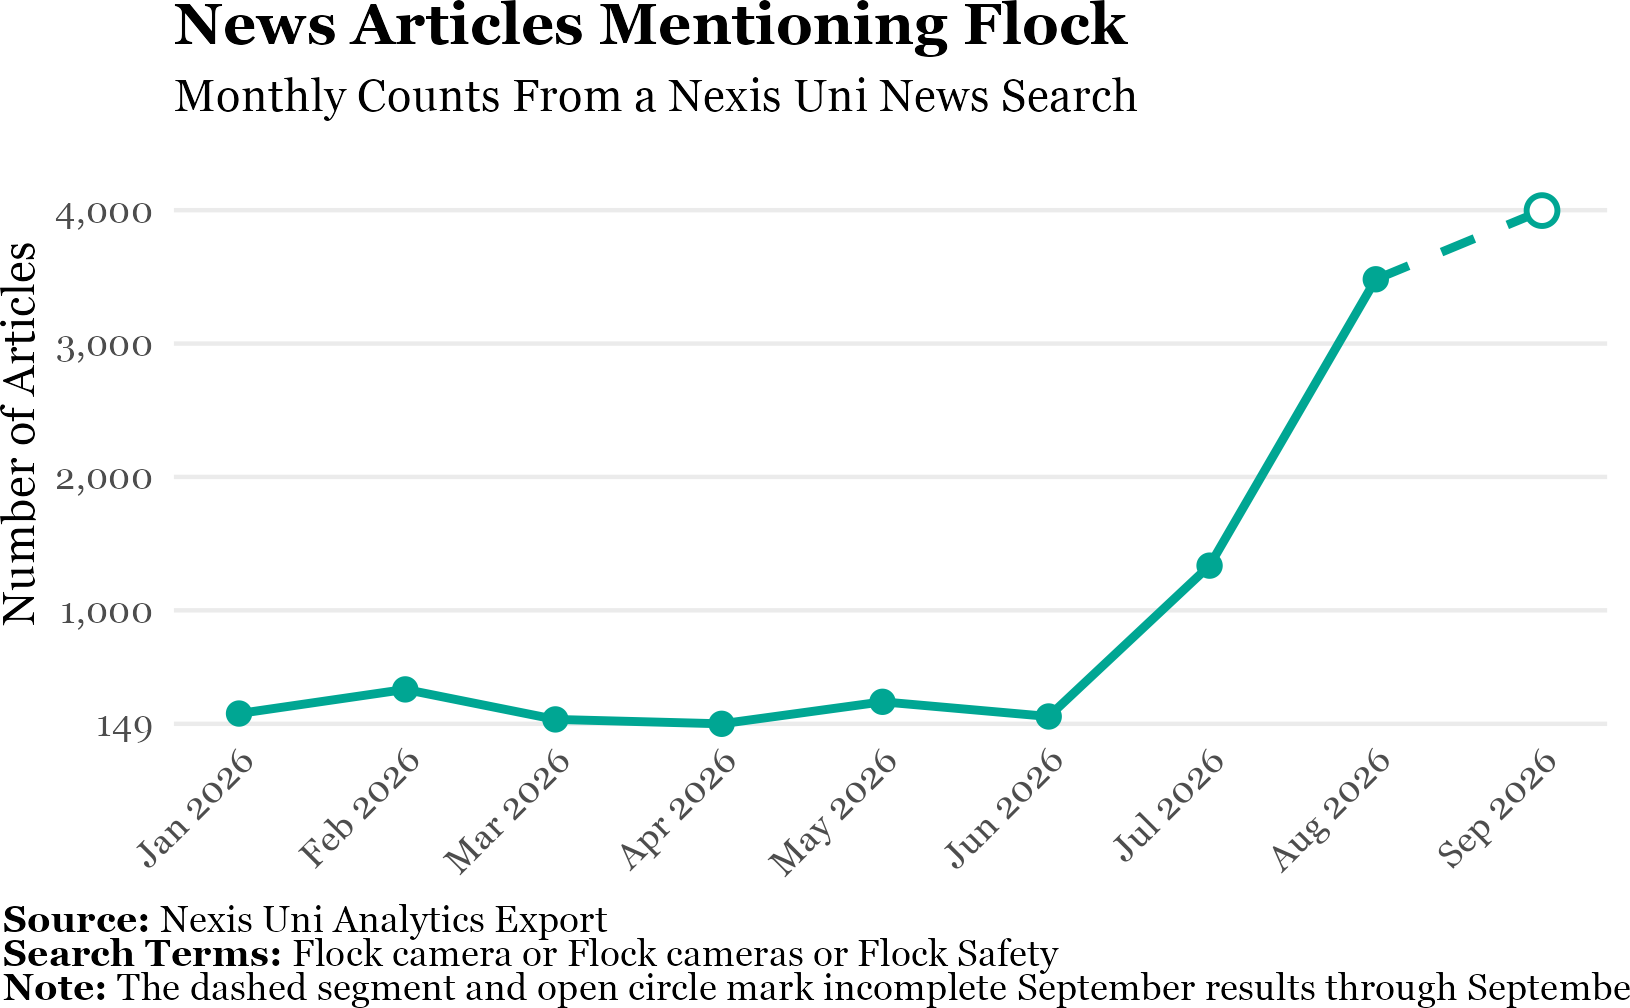
\includegraphics[keepaspectratio]{CMOS_18_UNIVERSAL_QUARTO_TEMPLATE_files/figure-pdf/unnamed-chunk-2-1.png}}

\begin{Shaded}
\begin{Highlighting}[]
\FunctionTok{ggsave}\NormalTok{(}
  \FunctionTok{file.path}\NormalTok{(}\FunctionTok{dirname}\NormalTok{(DATA\_FILE), }\StringTok{"Coverage\_Over\_Time\_Monthly.png"}\NormalTok{),}
  \AttributeTok{plot =}\NormalTok{ plot\_lexis\_coverage\_monthly,}
  \AttributeTok{width =} \FloatTok{8.88}\NormalTok{,}
  \AttributeTok{height =} \FloatTok{5.5}\NormalTok{,}
  \AttributeTok{units =} \StringTok{"in"}\NormalTok{,}
  \AttributeTok{dpi =} \DecValTok{300}\NormalTok{,}
  \AttributeTok{device =}\NormalTok{ ragg}\SpecialCharTok{::}\NormalTok{agg\_png}
\NormalTok{)}
\end{Highlighting}
\end{Shaded}

\begin{Shaded}
\begin{Highlighting}[]
\CommentTok{\# https://trends.google.com/explore?q=flock\&date=2026{-}01{-}01\%202026{-}09{-}27\&geo=US}

\NormalTok{DATA\_FILE2 }\OtherTok{\textless{}{-}} \StringTok{"time\_series\_US\_20260101{-}0000\_20260927{-}1417.csv"}

\NormalTok{google\_trends\_raw }\OtherTok{\textless{}{-}} \FunctionTok{read.csv}\NormalTok{(}
\NormalTok{  DATA\_FILE2,}
  \AttributeTok{check.names =} \ConstantTok{FALSE}\NormalTok{,}
  \AttributeTok{fileEncoding =} \StringTok{"UTF{-}8{-}BOM"}
\NormalTok{)}

\NormalTok{google\_trends\_weekly }\OtherTok{\textless{}{-}} \FunctionTok{data.frame}\NormalTok{(}
  \AttributeTok{week =} \FunctionTok{as.Date}\NormalTok{(google\_trends\_raw[[}\StringTok{"Time"}\NormalTok{]]),}
  \AttributeTok{search\_interest =} \FunctionTok{as.integer}\NormalTok{(google\_trends\_raw[[}\StringTok{"flock"}\NormalTok{]])}
\NormalTok{)}

\NormalTok{google\_trends\_weekly\_by\_day }\OtherTok{\textless{}{-}} \FunctionTok{do.call}\NormalTok{(}
\NormalTok{  rbind,}
  \FunctionTok{lapply}\NormalTok{(}\FunctionTok{seq\_len}\NormalTok{(}\FunctionTok{nrow}\NormalTok{(google\_trends\_weekly)), }\ControlFlowTok{function}\NormalTok{(i) \{}
    \FunctionTok{data.frame}\NormalTok{(}
      \AttributeTok{date =} \FunctionTok{seq}\NormalTok{(}
\NormalTok{        google\_trends\_weekly}\SpecialCharTok{$}\NormalTok{week[i],}
\NormalTok{        google\_trends\_weekly}\SpecialCharTok{$}\NormalTok{week[i] }\SpecialCharTok{+} \DecValTok{6}\NormalTok{,}
        \AttributeTok{by =} \StringTok{"day"}
\NormalTok{      ),}
      \AttributeTok{search\_interest =}\NormalTok{ google\_trends\_weekly}\SpecialCharTok{$}\NormalTok{search\_interest[i]}
\NormalTok{    )}
\NormalTok{  \})}
\NormalTok{)}

\NormalTok{google\_trends\_weekly\_by\_day }\OtherTok{\textless{}{-}} \FunctionTok{subset}\NormalTok{(}
\NormalTok{  google\_trends\_weekly\_by\_day,}
\NormalTok{  date }\SpecialCharTok{\textgreater{}=} \FunctionTok{as.Date}\NormalTok{(}\StringTok{"2026{-}01{-}01"}\NormalTok{) }\SpecialCharTok{\&}
\NormalTok{    date }\SpecialCharTok{\textless{}=} \FunctionTok{as.Date}\NormalTok{(}\StringTok{"2026{-}09{-}27"}\NormalTok{)}
\NormalTok{)}

\NormalTok{google\_trends\_weekly\_by\_day}\SpecialCharTok{$}\NormalTok{month }\OtherTok{\textless{}{-}} \FunctionTok{as.Date}\NormalTok{(}\FunctionTok{paste0}\NormalTok{(}
  \FunctionTok{format}\NormalTok{(google\_trends\_weekly\_by\_day}\SpecialCharTok{$}\NormalTok{date, }\StringTok{"\%Y{-}\%m"}\NormalTok{),}
  \StringTok{"{-}01"}
\NormalTok{))}

\NormalTok{google\_trends\_monthly }\OtherTok{\textless{}{-}} \FunctionTok{aggregate}\NormalTok{(}
\NormalTok{  search\_interest }\SpecialCharTok{\textasciitilde{}}\NormalTok{ month,}
  \AttributeTok{data =}\NormalTok{ google\_trends\_weekly\_by\_day,}
  \AttributeTok{FUN =}\NormalTok{ mean}
\NormalTok{)}

\NormalTok{google\_trends\_monthly}\SpecialCharTok{$}\NormalTok{month\_label }\OtherTok{\textless{}{-}} \FunctionTok{factor}\NormalTok{(}
  \FunctionTok{format}\NormalTok{(google\_trends\_monthly}\SpecialCharTok{$}\NormalTok{month, }\StringTok{"\%b \%Y"}\NormalTok{),}
  \AttributeTok{levels =} \FunctionTok{format}\NormalTok{(}
    \FunctionTok{seq}\NormalTok{(}\FunctionTok{as.Date}\NormalTok{(}\StringTok{"2026{-}01{-}01"}\NormalTok{), }\FunctionTok{as.Date}\NormalTok{(}\StringTok{"2026{-}09{-}01"}\NormalTok{), }\AttributeTok{by =} \StringTok{"month"}\NormalTok{),}
    \StringTok{"\%b \%Y"}
\NormalTok{  )}
\NormalTok{)}

\NormalTok{google\_trends\_complete\_months }\OtherTok{\textless{}{-}} \FunctionTok{subset}\NormalTok{(}
\NormalTok{  google\_trends\_monthly,}
\NormalTok{  month }\SpecialCharTok{\textless{}=} \FunctionTok{as.Date}\NormalTok{(}\StringTok{"2026{-}08{-}01"}\NormalTok{)}
\NormalTok{)}

\NormalTok{google\_trends\_september\_segment }\OtherTok{\textless{}{-}} \FunctionTok{subset}\NormalTok{(}
\NormalTok{  google\_trends\_monthly,}
\NormalTok{  month }\SpecialCharTok{\textgreater{}=} \FunctionTok{as.Date}\NormalTok{(}\StringTok{"2026{-}08{-}01"}\NormalTok{)}
\NormalTok{)}

\NormalTok{google\_trends\_september }\OtherTok{\textless{}{-}} \FunctionTok{subset}\NormalTok{(}
\NormalTok{  google\_trends\_monthly,}
\NormalTok{  month }\SpecialCharTok{==} \FunctionTok{as.Date}\NormalTok{(}\StringTok{"2026{-}09{-}01"}\NormalTok{)}
\NormalTok{)}

\NormalTok{plot\_google\_trends\_monthly }\OtherTok{\textless{}{-}} \FunctionTok{ggplot}\NormalTok{(}
\NormalTok{  google\_trends\_monthly,}
  \FunctionTok{aes}\NormalTok{(}\AttributeTok{x =}\NormalTok{ month\_label, }\AttributeTok{y =}\NormalTok{ search\_interest, }\AttributeTok{group =} \DecValTok{1}\NormalTok{)}
\NormalTok{) }\SpecialCharTok{+}
  \FunctionTok{geom\_line}\NormalTok{(}
    \AttributeTok{data =}\NormalTok{ google\_trends\_complete\_months,}
    \AttributeTok{color =} \StringTok{"\#00A693"}\NormalTok{,}
    \AttributeTok{linewidth =} \DecValTok{1}
\NormalTok{  ) }\SpecialCharTok{+}
  \FunctionTok{geom\_line}\NormalTok{(}
    \AttributeTok{data =}\NormalTok{ google\_trends\_september\_segment,}
    \AttributeTok{color =} \StringTok{"\#00A693"}\NormalTok{,}
    \AttributeTok{linewidth =} \DecValTok{1}\NormalTok{,}
    \AttributeTok{linetype =} \StringTok{"dashed"}
\NormalTok{  ) }\SpecialCharTok{+}
  \FunctionTok{geom\_point}\NormalTok{(}
    \AttributeTok{data =}\NormalTok{ google\_trends\_complete\_months,}
    \AttributeTok{color =} \StringTok{"\#00A693"}\NormalTok{,}
    \AttributeTok{size =} \FloatTok{2.3}
\NormalTok{  ) }\SpecialCharTok{+}
  \FunctionTok{geom\_point}\NormalTok{(}
    \AttributeTok{data =}\NormalTok{ google\_trends\_september,}
    \AttributeTok{color =} \StringTok{"\#00A693"}\NormalTok{,}
    \AttributeTok{fill =} \StringTok{"white"}\NormalTok{,}
    \AttributeTok{shape =} \DecValTok{21}\NormalTok{,}
    \AttributeTok{size =} \FloatTok{2.8}\NormalTok{,}
    \AttributeTok{stroke =} \DecValTok{1}
\NormalTok{  ) }\SpecialCharTok{+}
  \FunctionTok{scale\_x\_discrete}\NormalTok{(}
    \AttributeTok{drop =} \ConstantTok{FALSE}\NormalTok{,}
    \AttributeTok{expand =} \FunctionTok{expansion}\NormalTok{(}\AttributeTok{add =} \FloatTok{0.2}\NormalTok{)}
\NormalTok{  ) }\SpecialCharTok{+}
  \FunctionTok{scale\_y\_continuous}\NormalTok{(}
    \AttributeTok{breaks =} \FunctionTok{c}\NormalTok{(}\DecValTok{0}\NormalTok{, }\DecValTok{25}\NormalTok{, }\DecValTok{50}\NormalTok{, }\DecValTok{75}\NormalTok{, }\DecValTok{100}\NormalTok{),}
    \AttributeTok{limits =} \FunctionTok{c}\NormalTok{(}\DecValTok{0}\NormalTok{, }\DecValTok{100}\NormalTok{),}
    \AttributeTok{expand =} \FunctionTok{expansion}\NormalTok{(}\AttributeTok{mult =} \FunctionTok{c}\NormalTok{(}\DecValTok{0}\NormalTok{, }\DecValTok{0}\NormalTok{))}
\NormalTok{  ) }\SpecialCharTok{+}
  \FunctionTok{labs}\NormalTok{(}
    \AttributeTok{title =} \StringTok{"Google Search Interest in \textquotesingle{}flock\textquotesingle{}"}\NormalTok{,}
    \AttributeTok{subtitle =} \StringTok{"Monthly Averages of Weekly Scores in the United States"}\NormalTok{,}
    \AttributeTok{x =} \ConstantTok{NULL}\NormalTok{,}
    \AttributeTok{y =} \StringTok{"Relative Search Interest (0–100)"}\NormalTok{,}
    \AttributeTok{caption =} \FunctionTok{paste}\NormalTok{(}
      \StringTok{"\textless{}b\textgreater{}Source:\textless{}/b\textgreater{} Google Trends, United States"}\NormalTok{,}
      \StringTok{"\textless{}b\textgreater{}Search Term:\textless{}/b\textgreater{} flock"}\NormalTok{,}
      \StringTok{"\textless{}b\textgreater{}Method:\textless{}/b\textgreater{} Weekly scores are weighted by the days they cover in each month."}\NormalTok{,}
      \StringTok{"\textless{}b\textgreater{}Note:\textless{}/b\textgreater{} The dashed line and open circle mark September, which includes data through September 27, 2026."}\NormalTok{,}
      \AttributeTok{sep =} \StringTok{"\textless{}br\textgreater{}"}
\NormalTok{    )}
\NormalTok{  ) }\SpecialCharTok{+}
  \FunctionTok{theme\_minimal}\NormalTok{(}
    \AttributeTok{base\_family =} \StringTok{"Georgia"}\NormalTok{,}
    \AttributeTok{base\_size =} \DecValTok{11}
\NormalTok{  ) }\SpecialCharTok{+}
  \FunctionTok{theme}\NormalTok{(}
    \AttributeTok{plot.title =} \FunctionTok{element\_text}\NormalTok{(}\AttributeTok{face =} \StringTok{"bold"}\NormalTok{, }\AttributeTok{size =} \DecValTok{14}\NormalTok{),}
    \AttributeTok{axis.text.x =} \FunctionTok{element\_text}\NormalTok{(}\AttributeTok{angle =} \DecValTok{45}\NormalTok{, }\AttributeTok{hjust =} \DecValTok{1}\NormalTok{),}
    \AttributeTok{panel.grid.minor =} \FunctionTok{element\_blank}\NormalTok{(),}
    \AttributeTok{panel.grid.major.x =} \FunctionTok{element\_blank}\NormalTok{(),}
    \AttributeTok{plot.caption =}\NormalTok{ ggtext}\SpecialCharTok{::}\FunctionTok{element\_markdown}\NormalTok{(}\AttributeTok{hjust =} \DecValTok{0}\NormalTok{, }\AttributeTok{size =} \DecValTok{9}\NormalTok{),}
    \AttributeTok{plot.caption.position =} \StringTok{"plot"}
\NormalTok{  )}

\FunctionTok{print}\NormalTok{(plot\_google\_trends\_monthly)}
\end{Highlighting}
\end{Shaded}

\pandocbounded{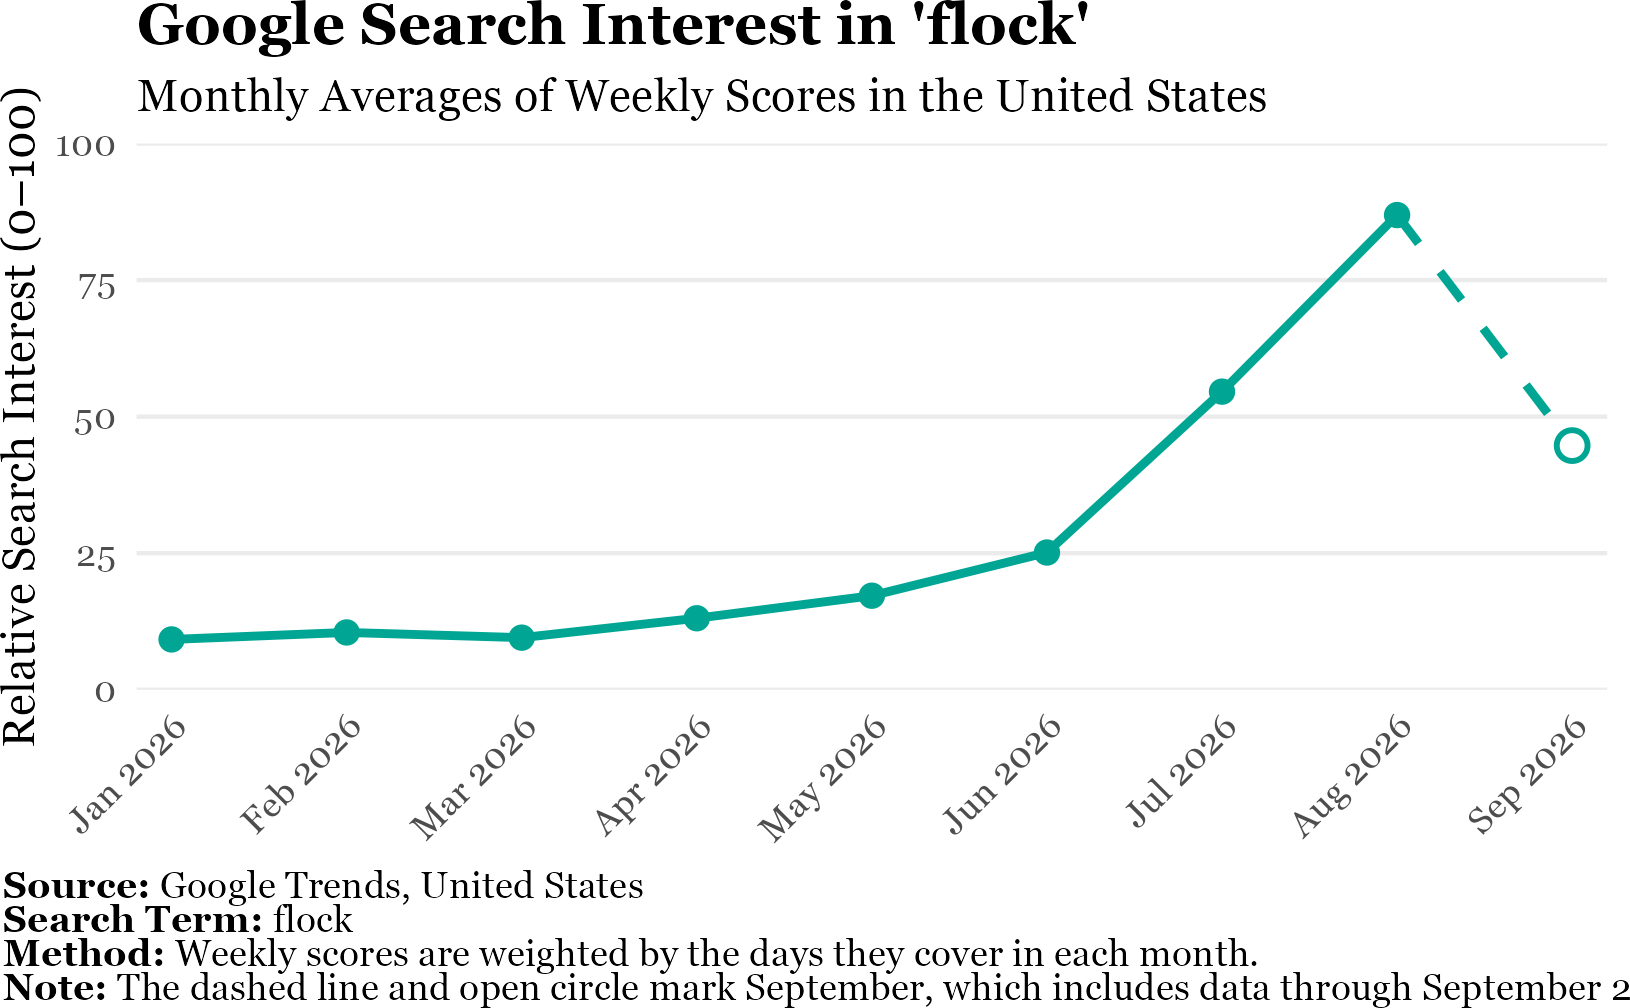
\includegraphics[keepaspectratio]{CMOS_18_UNIVERSAL_QUARTO_TEMPLATE_files/figure-pdf/unnamed-chunk-3-1.png}}

\begin{Shaded}
\begin{Highlighting}[]
\FunctionTok{ggsave}\NormalTok{(}
  \FunctionTok{file.path}\NormalTok{(}\FunctionTok{dirname}\NormalTok{(DATA\_FILE2), }\StringTok{"Google\_Search\_Interest\_Flock\_Monthly.png"}\NormalTok{),}
  \AttributeTok{plot =}\NormalTok{ plot\_google\_trends\_monthly,}
  \AttributeTok{width =} \FloatTok{8.88}\NormalTok{,}
  \AttributeTok{height =} \FloatTok{5.5}\NormalTok{,}
  \AttributeTok{units =} \StringTok{"in"}\NormalTok{,}
  \AttributeTok{dpi =} \DecValTok{300}\NormalTok{,}
  \AttributeTok{device =}\NormalTok{ ragg}\SpecialCharTok{::}\NormalTok{agg\_png}
\NormalTok{)}
\end{Highlighting}
\end{Shaded}

\section{Contemporary Literature}\label{contemporary-literature}

This demonstrates a Level 1 heading.

\subsection{What Are the Major
Movements?}\label{what-are-the-major-movements}

This demonstrates a Level 2 heading.

\subsubsection{Beat Generation}\label{beat-generation}

This demonstrates a Level 3 heading.

\paragraph{Significant figures, events, and
elements}\label{significant-figures-events-and-elements}

This demonstrates a Level 4 heading.

\emph{Kerouac as the leader.} The role of founding Beat Generation poet
was filled by Jack Kerouac. This Level 5 heading remains run-in across
the major output formats.

\section{Block Quotation Example}\label{block-quotation-example}

Normal double-spaced body text appears before the block quotation.

\begin{quote}
This is an example of a block quotation. A prose quotation of five or
more lines or more than one hundred words should be blocked. It begins
on a new line, appears without quotation marks, is indented from the
left margin, and is single-spaced. (Smith 2024, 50)
\end{quote}

Normal double-spaced body text resumes here.

\section{Conclusion}\label{conclusion}

Write your conclusion here.

\newpage

\begin{singlespace}

\noindent\makebox[\textwidth][c]{References}\par

% Two blank lines between heading and first entry.

\vspace{2\baselineskip}

\protect\phantomsection\label{refs}
\begin{CSLReferences}{1}{1}
\bibitem[\citeproctext]{ref-jones2022}
Jones, Maria L. 2022. {``Institutions, Public Opinion, and Political
Change.''} \emph{Journal of Social Research} 48 (3): 215--38.
\url{https://doi.org/10.0000/example.2022.001}.

\bibitem[\citeproctext]{ref-smith2024}
Smith, John A. 2024. \emph{Politics and Society in the Modern World}.
University of Chicago Press.

\end{CSLReferences}

\end{singlespace}




\end{document}
